% pdflatex HLA.tex
\documentclass[12pt]{article}

\usepackage{fullpage}
\usepackage{multicol, multirow}
\usepackage{tabularx}
\usepackage{graphicx}
\usepackage{ulem}
\usepackage[utf8]{inputenc}
\usepackage[russian]{babel}

\begin{document}

\begin{titlepage}

\newpage

% insert a title page here

\end{titlepage}
\tableofcontents{}



\newpage
\section{Высокоуровневая архитектура}
\subsection{Концепция}
Приложение является интернет-мессенджером для социальной сети <<Вконтакте>>. Оно позволяет отправлять и принимать текстовые сообщения пользователям из списка друзей, подгружать историю сообщений с сервера, а также уведомлять о новых сообщениях с помощью всплывающих окон и звуковых сигналов.

\subsection{Физическая архитектура}
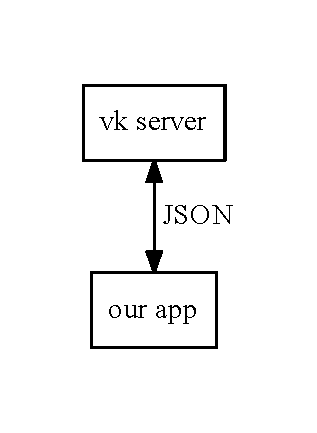
\includegraphics{../HLA/diag/phys.pdf}

\subsection{Логическая архитектура}
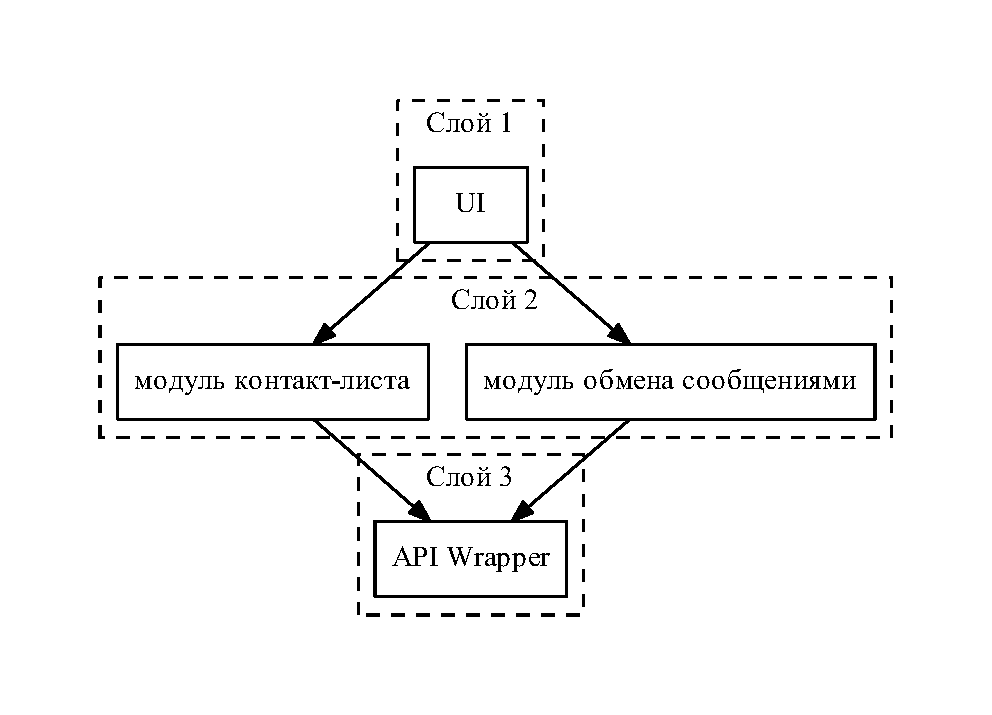
\includegraphics{../HLA/diag/logic.pdf}

\subsection{Нефункциональные требования}

\subsubsection{Производительность}
Время отправки/получения сообщений, если они есть на сервере, при стабильном интернет-соединении (ping до vk.com < 100 ms) — в диапазоне от 1 до 2 c (в общем случае зависит от настроек).

\subsubsection{Сопровождаемость}
Самодокументируемый код, комментарии к неочевидным моментам. Логгирование ошибок в консоли Python. \\
Доступен репозиторий на GitHub (http://github.com/r3t/oop-project), где можно оставлять сообщения об ошибках и недочётах.

\subsubsection{Пользовательский интерфейс}
Главное окно со списком контактов; окно со вкладками чатов; всплывающие уведомления в углу экрана; окно конфигурации. Интерфейс минималистичен, требуемые подписи к элементам управления — на английском.

\subsubsection{Операционное окружение}
Кроссплатформенность: Windows, Linux, Mac OS и любая другая система, позволяющая работать с графическим интерфейсом и имеющая интерпретатор языка Python.

\subsubsection{Безопасность}
Пароль пользователя нигде не хранится ни в явном, ни в шифрованном виде. Для авторизации используется протокол на базе OAuth 2.0.
Пользователь разрешает приложению доступ к своим данным. В приложение передается ключ $access\_token$ для доступа к API.

\subsection{Компоненты и инструменты} 
\begin{enumerate}
\item Python 2.7.X
\item PyQt 4.10.3+
\item vkontakte 1.3.2 (vk.com (aka vkontakte.ru) API wrapper)
\end{enumerate}



\newpage
\section{Распределение ролей}
\subsection{Ильвохин Дмитрий}
\begin{itemize}
\setlength{\itemsep}{-1mm} % уменьшает расстояние между элементами списка
\item Диаграммы HLA
\item Интерфейс и логика работы главного окна, окна логина, всплывающих окон
\item Работа с API
\item Работа с потоками
\item Реализация шаблонов <<Реестр>>, <<Фасад>> и обработки ошибок (шаблон <<Декоратор>>)
\end{itemize}

\subsection{Данилычев Иван}
\begin{itemize}
\setlength{\itemsep}{-1mm}
\item Интерфейс и логика работы окна и вкладок сообщений, окна настроек
\item Функционал окна сообщений
\item Ресурсы приложения (иконки)
\end{itemize}



\newpage
\section{Примененные шаблоны проектирования}
\subsection{Реестр}
В реестре (класс {\tt Registry}) хранятся единичные экземпляры объектов, к которым требуется доступ из, возможно, любого модуля. Такими объектами стали:
\begin{itemize}
\setlength{\itemsep}{-1mm} % уменьшает расстояние между элементами списка
\item Конфигурация приложения. Она существует в единственном числе, при этом, помимо главного окна, требуется во вкладках сообщений и, собственно, самого окна настроек.
\item Обертка над классом, работающим с API, поскольку клиент сообщений однопользовательский.
\end{itemize}

\subsection{Фасад}
Фасад (класс {\tt VkClientThread}) служит посредником между обёрткой и главным окном. Он хранит в себе некоторые результаты последних запросов к API, а также распределяет их по компонентам приложения с помощью потоков, каждый из которых отвечает за свои типы запросов. Таким образом, фасад снимает постоянную или частую нагрузку с интерфейса, позволяя приложению реагировать на действия пользователя.

\subsection{Декоратор}
Декоратор, реализованный с помощью встроенных в Python декораторов, выступет в виде надстройки над функциями для работы с сетью при обращении к API.



\section{Схема работы класса VkClientThread}
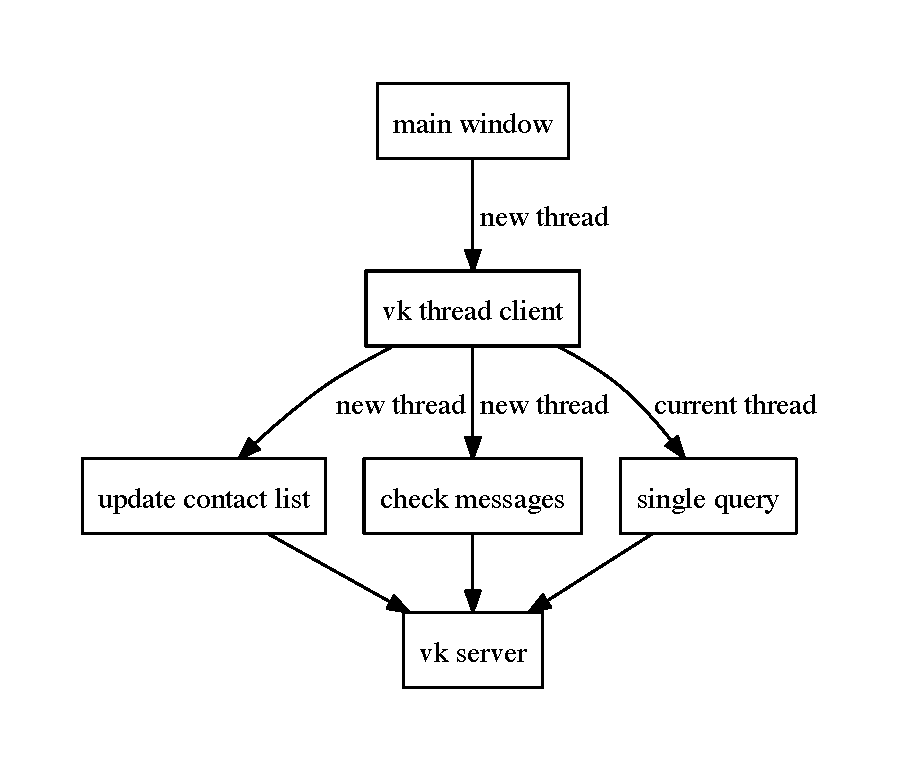
\includegraphics{./diag/work_logic.pdf}



\newpage
\section{Модульное тестирование}
\subsection{Инструменты}

Для модульного тестирования используется стандартный модуль языка Python --- unittest.

\subsection{Тесты}
\subsection{Тестирование класса VkClientThread}
При тестировании проверяются следующие возможности:
\begin{itemize}
\setlength{\itemsep}{-1mm}
\item Отправка сообщений,
\item Прием сообщений,
\item Пометка сообщений прочитанными.
\end{itemize}

\subsubsection{Сценарий тестирования}
\begin{itemize}
\setlength{\itemsep}{-1mm}
\item Отправим сообщение самому себе;
\item Получим непрочитанные сообщения, проверим, что отправленное сообщение есть в полученных;
\item Отметим сообщение прочитанным, проверим, что число непрочитанных сообщений уменьшилось;
\end{itemize}

\subsection{Тестирование класса Config}
При тестировании проверяются следующие возможности:
\begin{itemize}
\setlength{\itemsep}{-1mm}
\item Правильность начальной конфигурации,
\item Правильность добавления данных и обновления состояния.
\end{itemize}

\subsection{Тестирование подсветки ссылок}
При тестировании проверяется корректная обработка протоколов для случаев, когда протокол один или их несколько.



\newpage
\section{Функциональное тестирование}
\subsection{Тест-кейс 1: проверка уведомлений}
\begin{itemize}
\setlength{\itemsep}{-1mm}
\item Запустить приложение, залогиниться;
\item Получить несколько сообщений подряд от одного из друзей, не читая их. Проверить наличие поп-апов и их корректность (напр., отсутствие иконки в панели окон), а также наличие звукового уведомления;
\item Закрыть и вновь запустить приложение; проверить, что при запуске приходят уведомления о непрочитанных сообщениях, а при клике по ним левой кнопкой мыши открывается окно чата;
\item Завершить тестирование.
\end{itemize}

\subsection{Тест-кейс 2: получение новых сообщений и работа с вкладками}
\begin{itemize}
\setlength{\itemsep}{-1mm}
\item Запустить приложение, залогиниться;
\item Открыть вкладку чата с одним из друзей, сделать её неактивной;
\item При получении сообщения проверить, что на вкладке рядом с именем собеседника появляется иконка конверта, поп-ап, а также воспроизводится звуковое уведомление;
\item Проверить, что при клике в область чата или набора сообщения значок исчезает; кроме того, проверить, что при активном окне уведомлений не поступает;
\item Проверить, что уведомления появляются, если в данный момент активна другая вкладка.
\item Проверить, что существующие вкладки корректно делают себя текущими активными окнами, а также перехватывают фокус клавиатуры при переключении и попытке повторного открытия;
\item Завершить работу.
\end{itemize}

\subsection{Тест-кейс 3: отправка сообщений}
\begin{itemize}
\setlength{\itemsep}{-1mm}
\item Запустить приложение, залогиниться;
\item Открыть вкладку чата с одним из друзей;
\item Отправить собеседнику несколько сообщений;
\item Проверить каким-либо способом (например, через веб-версию чата), что сообщения доставлены;
\item Завершить работу.
\end{itemize}

\subsection{Тест-кейс 4: обновление настроек}
\begin{itemize}
\setlength{\itemsep}{-1mm}
\item Запустить приложение, залогиниться;
\item Начать разговор с кем-нибудь из друзей;
\item Открыть окно конфигурации, поменять несколько параметров, в т. ч. отвечающих за связь с сервером;
\item Закрыть окно чата и открыть повторно;
\item Удостовериться, что некоторые детали интерфейса приложения изменились, следуя новой конфигурации;
\item Завершить работу.
\end{itemize}



\newpage
\section{Выводы}
\indent При разработке клиента сообщений очень пригодились такие шаблоны проектирования, как реестр и фасад: первый упростил взаимодействие между классами, избавив их, а заодно и разработчиков, от проблемы постоянного обмена одними и теми же объектами и контроля их единственности. Фасад облегчил работу со сторонней библиотекой, объединив запросы к серверу и контроль актуальности получаемых ответов. Кроме того, за счёт некоторого усложнения логики фасада была облегчена логика основного приложения: фасад сам сигнализирует о наличии необходимых данных, используя концепцию сигналов и слотов библиотеки (Py)Qt. \newline

На проектировании и логике работы сильно сказалась зависимость от сервера. Первоначальная версия приложения при любом запросе к API ВКонтакте <<замораживала>> интерфейс, в связи с чем потребовались отдельные потоки для запросов. Помимо нашего мессенджера, к серверу подключается множество других пользователей, в связи с чем некоторые потоки время от времени получают вместо реального ответа сообщение о таймауте запроса (и не только). Чтобы связь не терялась неявно, был написан отдельный класс-декоратор, устанавливающий соединение и передающий его дальше по коду, обрабатывая таким образом исключения. Кроме того, он выводит в консоль лог пойманных исключений. \newline

Повлияло наличие сервера также и на процесс тестирования. Поскольку контролировать получаемые данные, как и эмулировать работу сервера, оказалось затруднительно, основная работа пришлась на тестирование функционала приложения и составление тест-кейсов. Модульное тестирование было проведено лишь для немногих самостоятельных внутренних компонентов, к примеру, класса конфигурации.

В заключение стоит сказать о недостатках и возможном улучшении приложения. К примеру, поддерживаются далеко не все функции работы со списком контактов (удаление, просмотр личных данных). Также заметна неполнота многопоточности: при отправке сообщения адресату приложение на секунду <<подвисает>>.
\end{document}
